This section outlines the User Interface of the S\&C system, providing an overview of the various pages that form the core of the platform. The design mockups presented in this document focus on interaction dynamics and functionality rather than the final visual aesthetics, acknowledging that graphical elements may undergo adjustments during the testing and refinement phases. While the desktop browser version is emphasized due to its alignment with the platform's primary objective of connecting students and companies, equivalent pages will be designed and optimized for the mobile version to ensure a seamless and responsive user experience across devices.

As highlighted in the RASD, these design mockups serve as an initial representation of the interface and are subject to iterative enhancements based on testing outcomes and user feedback, ensuring that the system meets the expectations of its target audience while maintaining usability and efficiency.


\section{Overview}

\begin{figure}[H]
    \begin{center}
        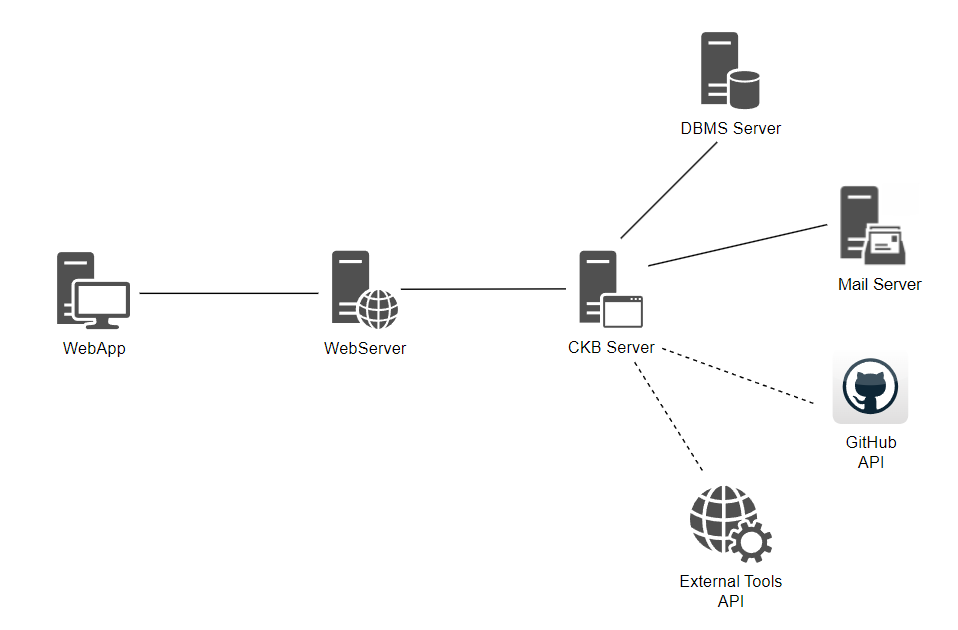
\includegraphics[width=0.8\linewidth]{Interfaces_UI/Overview.png}
        \caption{User Interface Overview.}
        \label{fig:user_interface_overview}%
    \end{center}
\end{figure}

The provided diagram presents a comprehensive overview of the S\&C system’s pages, illustrating their interconnections and the primary pathways for user navigation. Each page serves a specific purpose in enabling seamless interaction between students and companies. Detailed descriptions of each page are provided in the following sections, with the exception of the landing page, which is implicit as it primarily serves as an introduction to the platform and provides access to the login and registration pages.


\section{Header}

\begin{figure}[H]
    \begin{center}
        
\includegraphics[width=1\linewidth]{Interfaces_UI/Header.png}
        \caption{Header.}
        \label{fig:header}%
    \end{center}
\end{figure}

Across all pages in the S\&C system, a uniform header ensures a consistent and user-friendly experience. The header prominently displays the platform name, a notification icon to keep users updated, a menu icon for easy navigation, and the user’s name or identifier. These elements provide quick access to essential features, enhancing usability across the platform.

In cases where the user is a company or a university, the header undergoes slight modifications to better cater to their role. For instance, instead of the user's name, the company or institution’s name is displayed, reflecting their organizational identity. Additionally, the menu options adapt to include functionalities specific to these users, such as "Recommended Students" or "Create Tasks." Despite these changes, the cohesive design of the header remains consistent, ensuring familiarity and accessibility for all users.
 

\newpage

\section{User Interfaces}
\newcounter{ui}
\setcounter{ui}{1}
\newcommand{\cui}{\theui\stepcounter{ui}}

\subsection*{UI\cui . Login and Registration Pages}

\begin{figure}[H]
    \begin{center}
        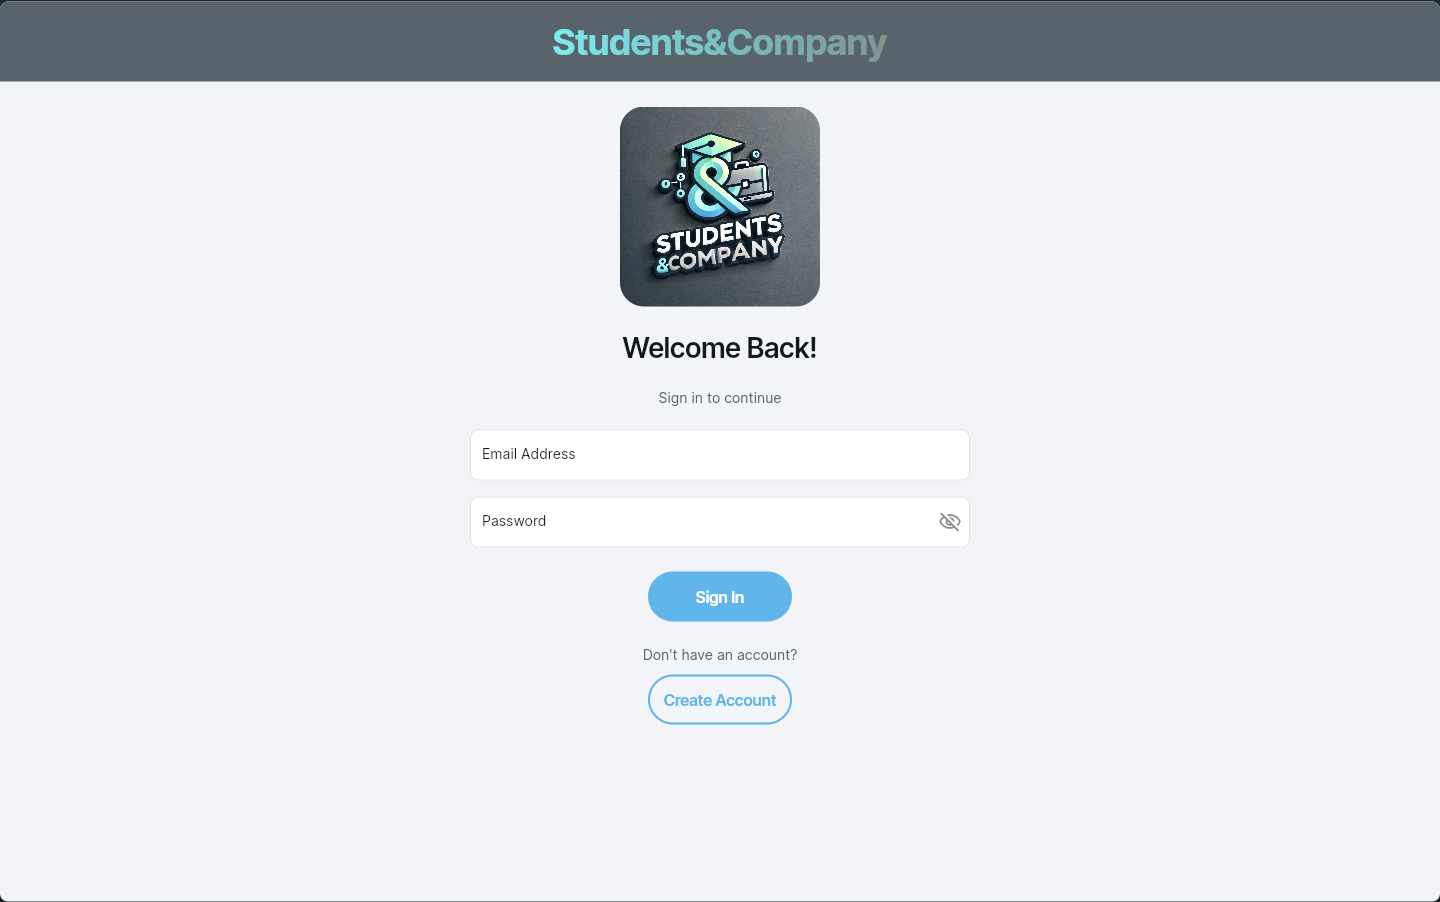
\includegraphics[width=0.7\linewidth]{Interfaces_UI/LoginPage.png}
        \caption{Login Page.}
        \label{fig:login_page}%
    \end{center}

    \begin{center}
        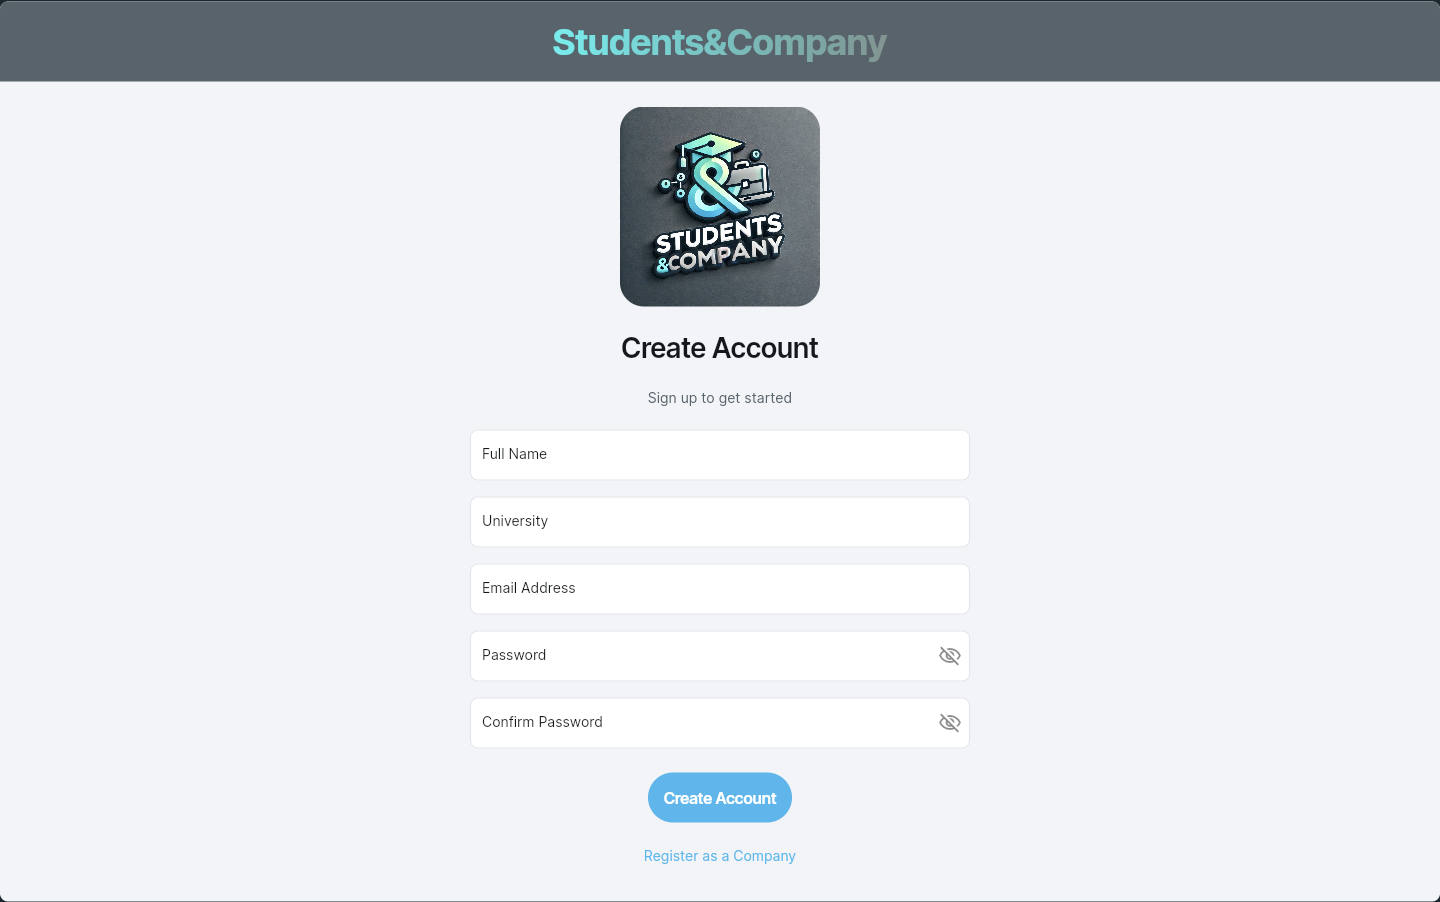
\includegraphics[width=0.7\linewidth]{Interfaces_UI/RegistrationPage.png}
        \caption{Registration Page.}
        \label{fig:registration_page}%
    \end{center}
\end{figure}

Description 

\subsection*{UI\cui . ST Homepage}

\begin{figure}[H]
    \begin{center}
        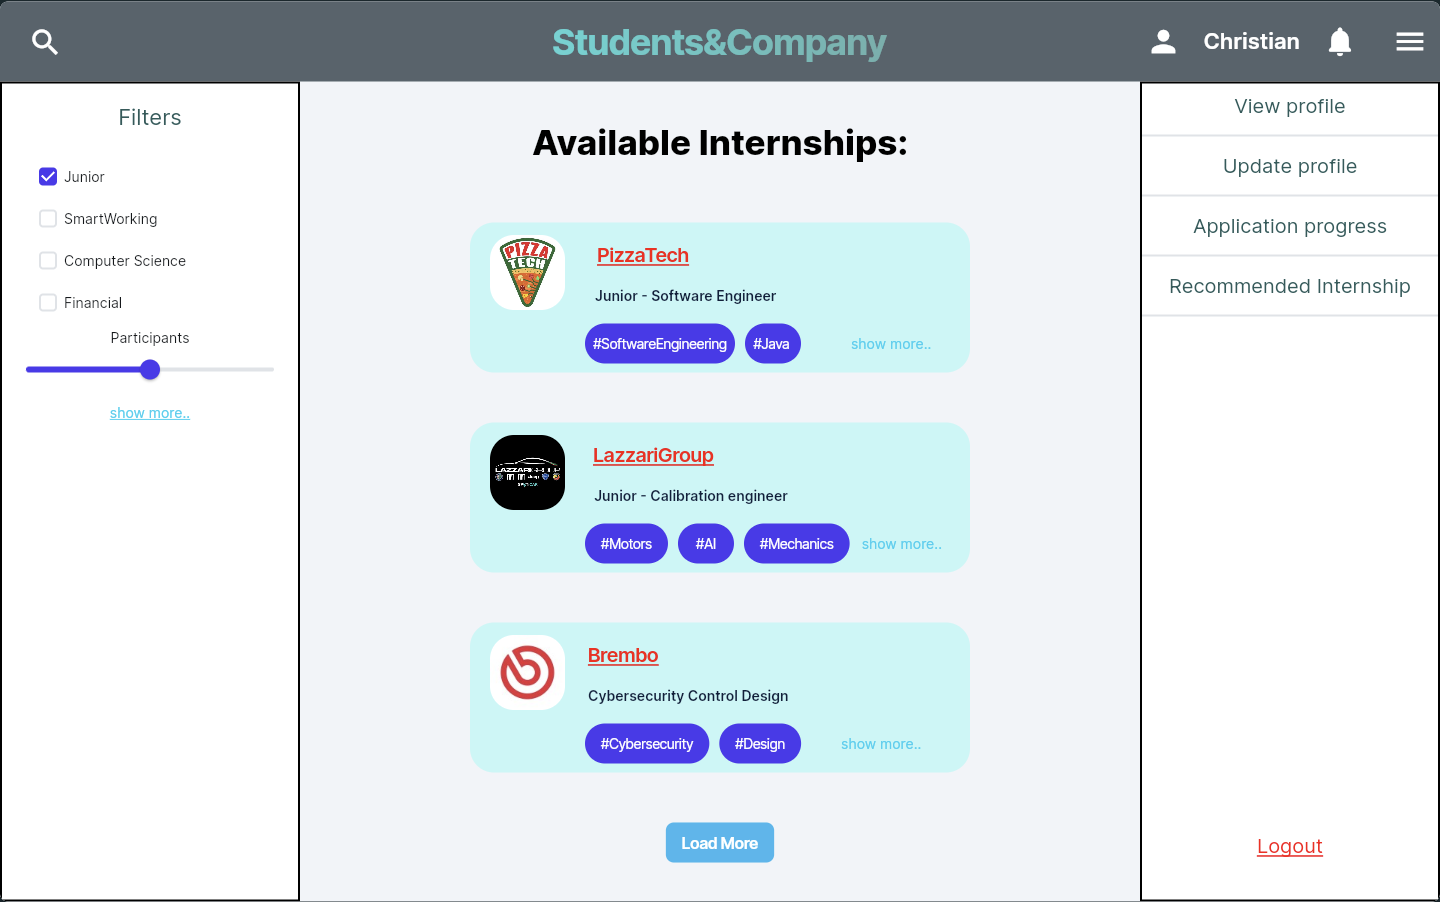
\includegraphics[width=0.7\linewidth]{Interfaces_UI/STHomePage.png}
        \caption{ST Homepage.}
        \label{fig:st_homepage}%
    \end{center}
\end{figure}

Description

\subsection*{UI\cui . Update Profile Page}

\begin{figure}[H]
    \begin{center}
        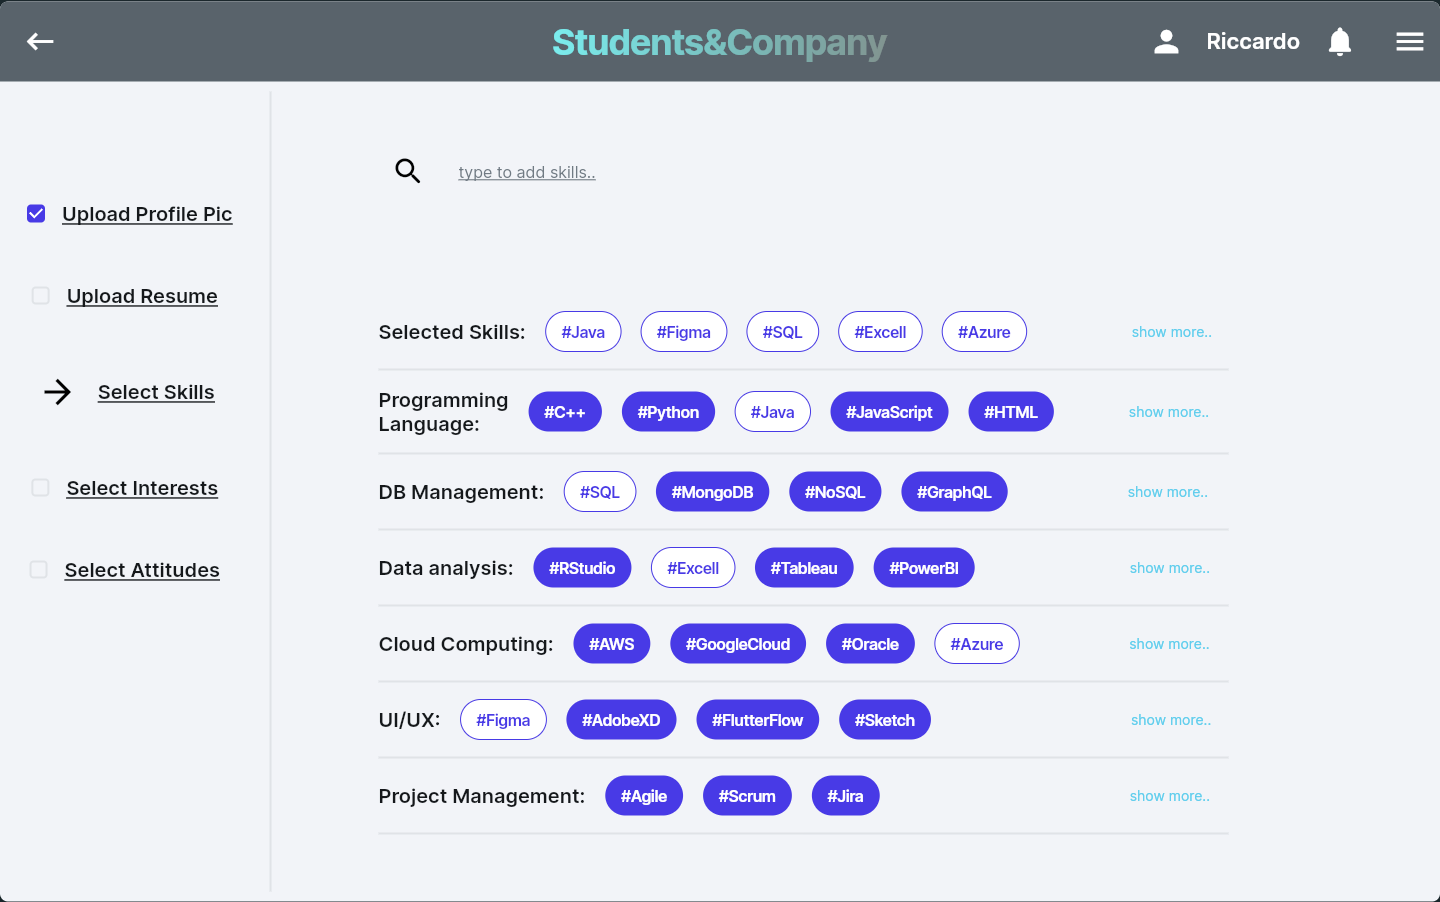
\includegraphics[width=0.7\linewidth]{Interfaces_UI/UpdateProfilePage.png}
        \caption{Update Profile Page.}
        \label{fig:update_profile_page}%
    \end{center}
\end{figure}

Description

\subsection*{UI\cui . CP Homepage}

\begin{figure}[H]
    \begin{center}
        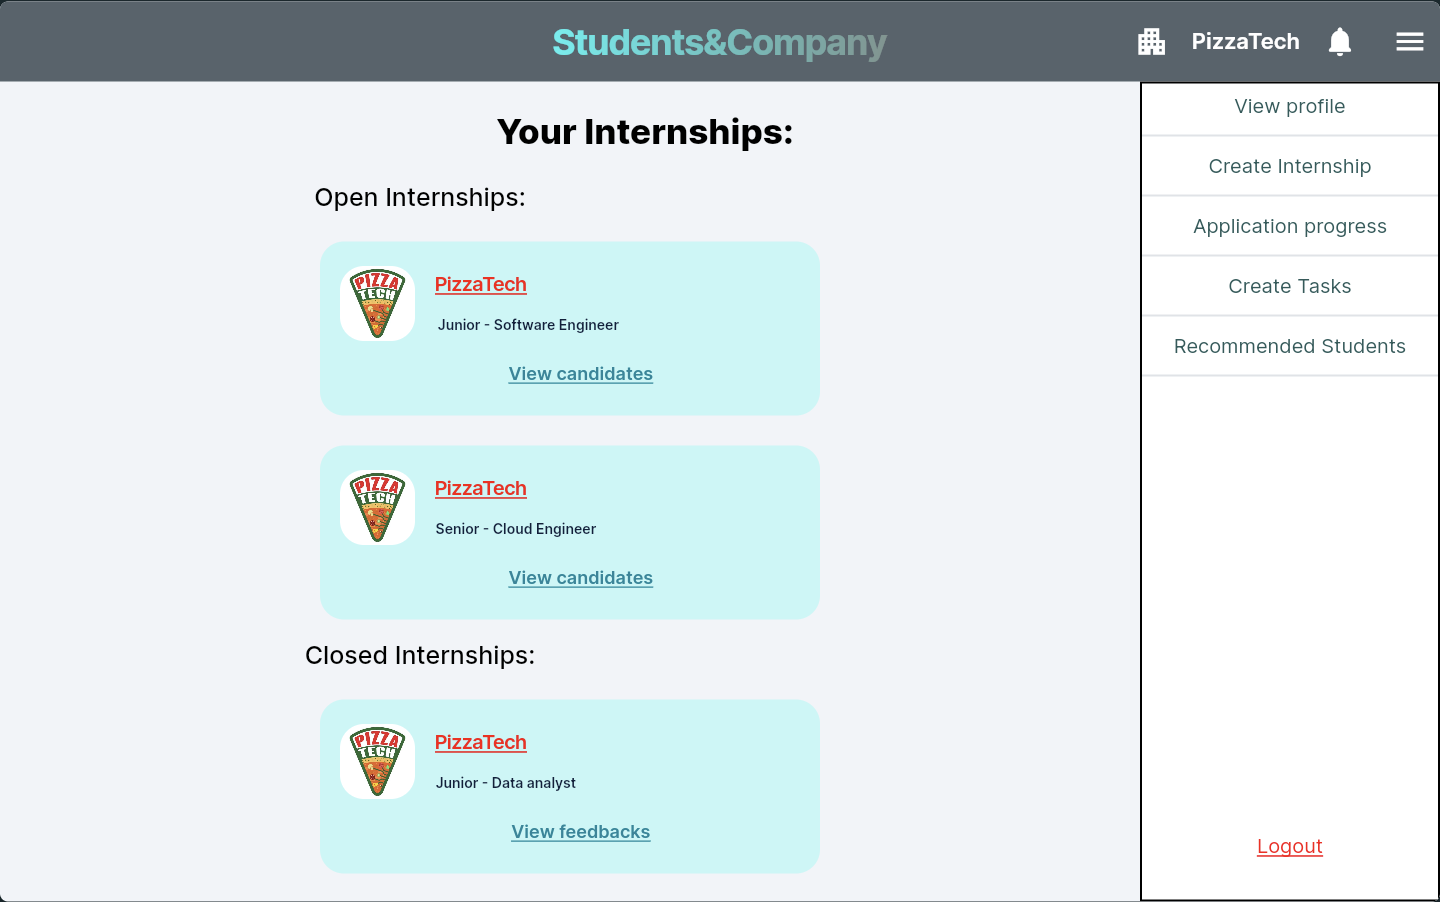
\includegraphics[width=0.7\linewidth]{Interfaces_UI/CPHomePage.png}
        \caption{CP Homepage.}
        \label{fig:company_homepage}%
    \end{center}
\end{figure}

Description

\subsection*{UI\cui . Create Internship Page}

\begin{figure}[H]
    \begin{center}
        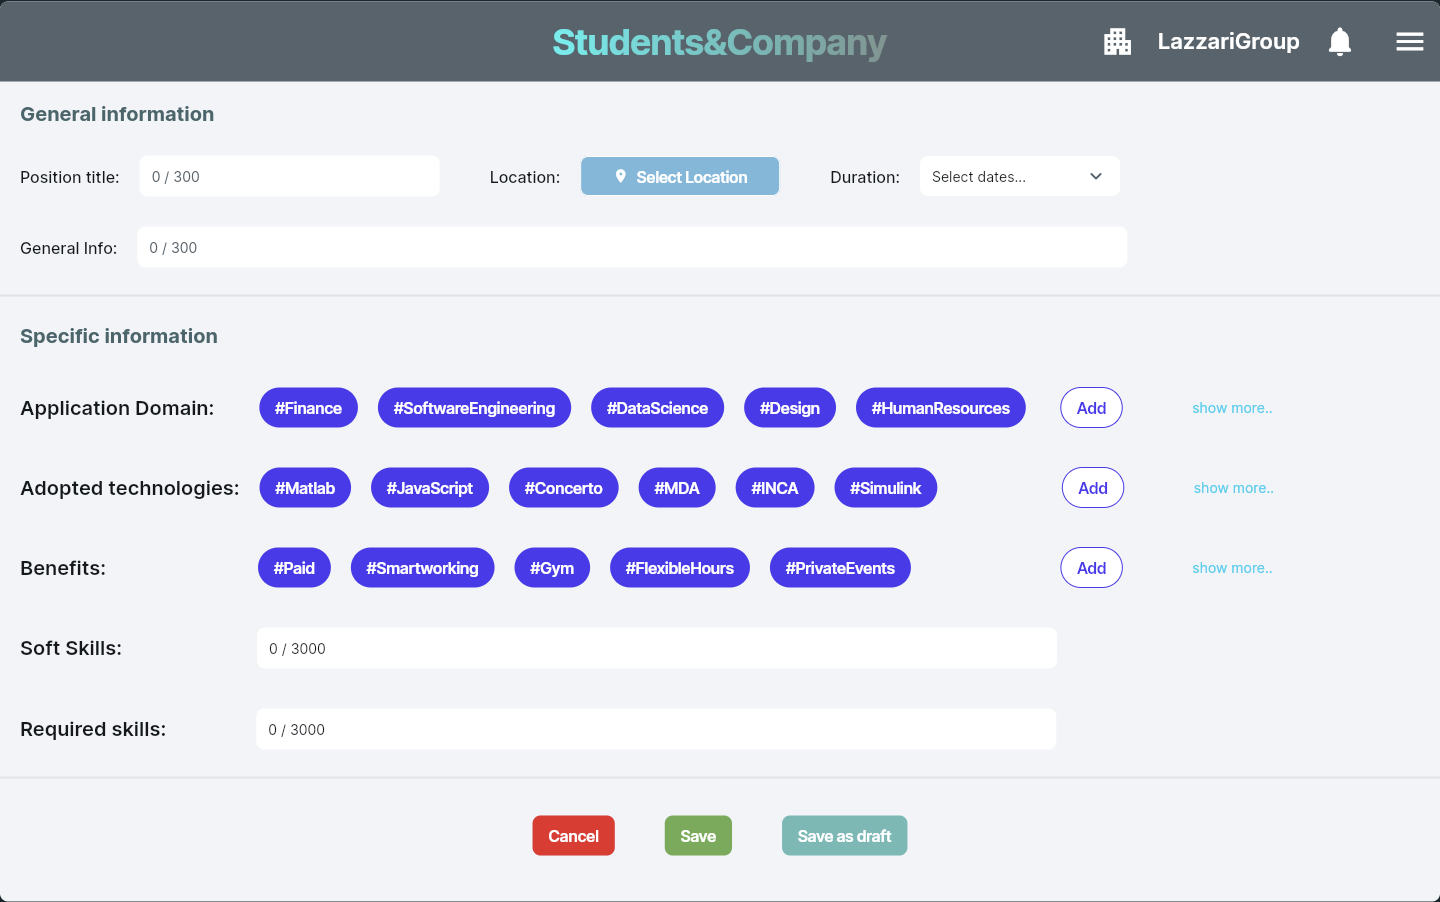
\includegraphics[width=0.7\linewidth]{Interfaces_UI/CreateInternshipPage.png}
        \caption{Create Internship Page.}
        \label{fig:create_internship_page}%
    \end{center}   
\end{figure}

Description

\subsection*{UI\cui . View Profile Page}

\begin{figure}[H]
    \begin{center}
        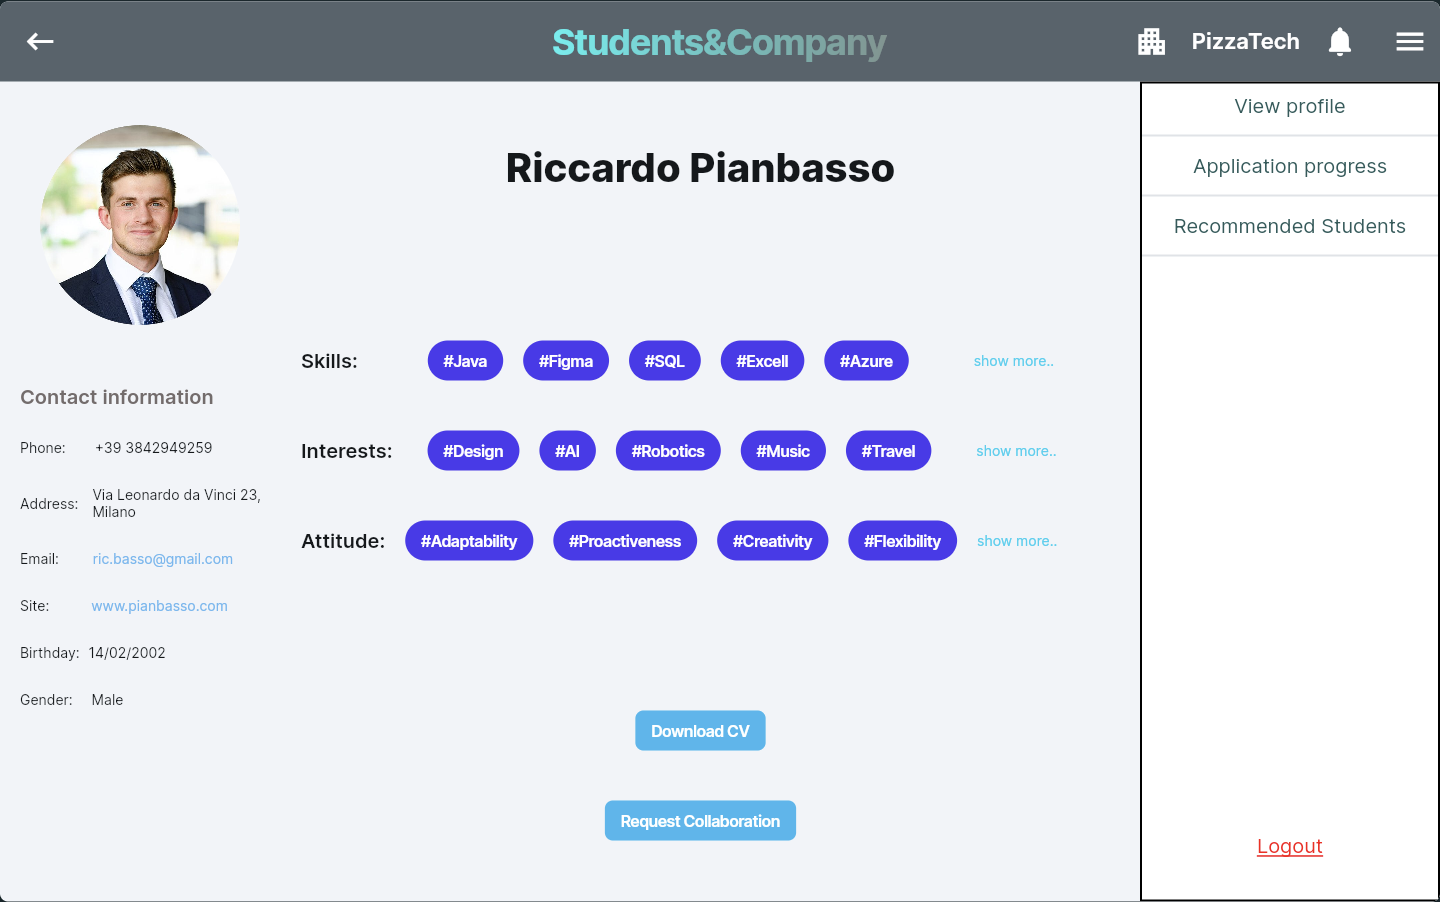
\includegraphics[width=0.7\linewidth]{Interfaces_UI/ViewProfilePage.png}
        \caption{View Profile Page.}
        \label{fig:view_profile_page}%
    \end{center}
\end{figure}

Description

\subsection*{UI\cui . View Internship Page}

\begin{figure}[H]
    \begin{center}
        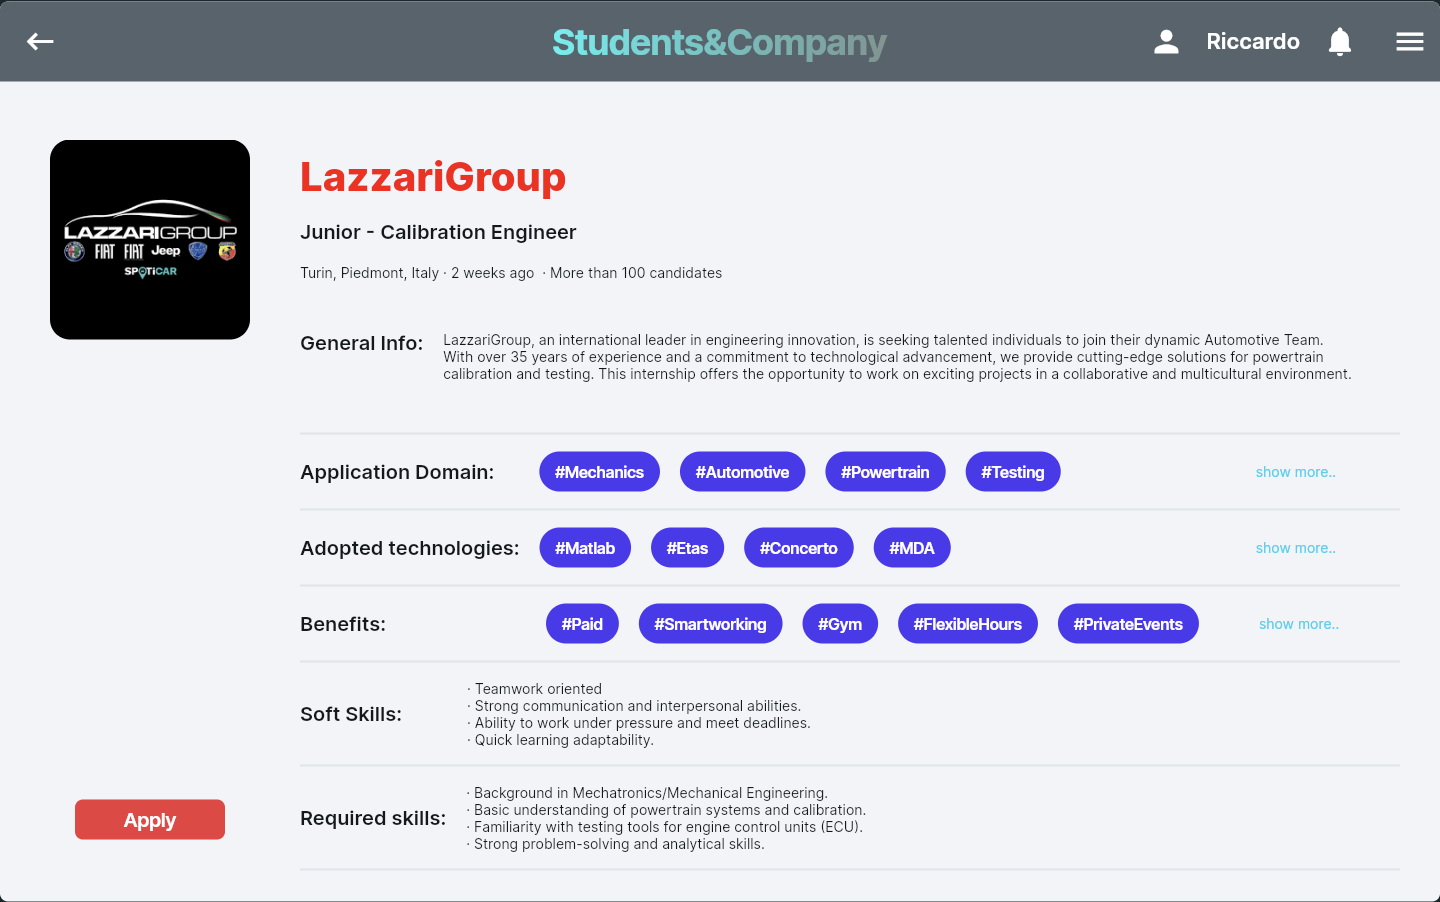
\includegraphics[width=0.7\linewidth]{Interfaces_UI/ViewInternshipPage.png}
        \caption{View Internship Page.}
        \label{fig:view_internship_page}%
    \end{center}
\end{figure}

Description

\subsection*{UI\cui . Application Progress Page}

\begin{figure}[H]
    \begin{center}
        \includegraphics[width=0.7\linewidth]{Interfaces_UI/applicationProgressPage.png}
        \caption{Application Progress Page.}
        \label{fig:application_progress_page}%
    \end{center}   
\end{figure}

Description 




